\subsection{Remote control block}\label{chapter_REMOTE_CONTROL_BLOCK}
This chapter will show the 'innards' of the first block, pictured in cyan in Figure \ref{fig:MATLAB Overview}.
\begin{figure}[H]
	\centering
		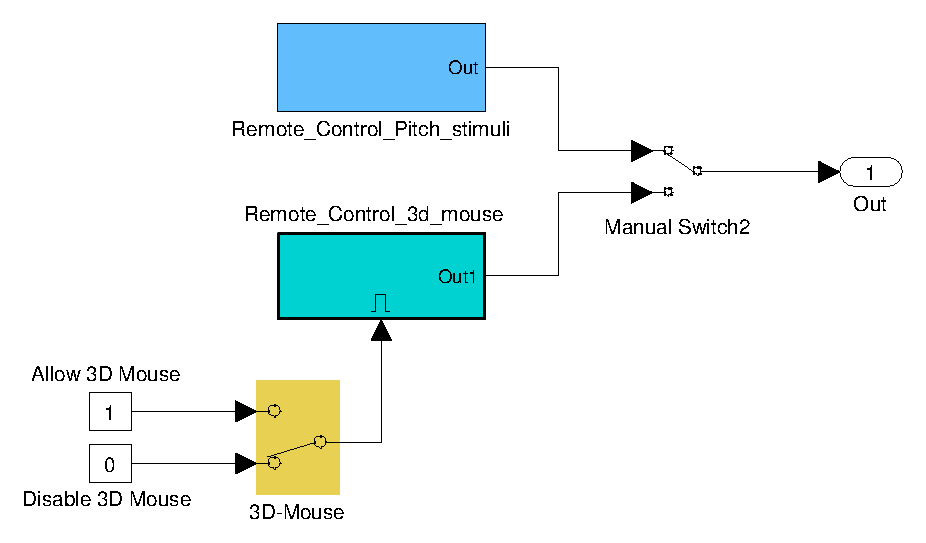
\includegraphics[width=0.8\textwidth]{03_Grafiken/MATLAB_Remote_Control_Overview.pdf}
	\caption{Remote control block overview}
	\label{fig:Remote control block}
\end{figure}
The cyan block in this figure, allows to connect a 3D-mouse to the computer to steer the quadrocopter in the animation. This research paper doesn't elaborate on this block.
The block in light-blue allows to generate manual stimuli. The content of this block is showed below.
\begin{figure}[htbp]
	\begin{minipage}[t]{6cm}
		\vspace{0pt}
		\centering
		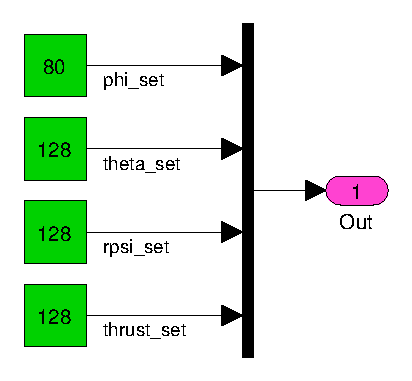
\includegraphics[width=6cm]{03_Grafiken/MATLAB_Remote_Control_Stimuli.pdf}
		\caption{Stimuli}
		\label{fig:Remote control stimuli}
	\end{minipage}
	\hfill
	\begin{minipage}[t]{8cm}
		\vspace{0pt}
		\medskip
		\begin{onehalfspace}
		By double clicking the green blocks, it is possible to change the values of these blocks. The values range 		 
		from 0 to 255, where 128 means angle zero for phi (roll) and theta (pitch) or rather angular rate zero for 			rate of psi (yaw rate). Value 255 of thrust means 				
		full-speed to all motors.
		So the stimuli in the left figure say 'no pitching, no yaw rate and a negative angle towards the horizontal 	
		(roll left) at half thrust'.
		\end{onehalfspace}
	\end{minipage}
\end{figure}